\documentclass[12pt]{article}
\usepackage[utf8]{inputenc}
\usepackage[figures]{updiplom}
\usepackage{epstopdf,graphicx,dsfont}
\usepackage{listings}%zdrojove kody
\usepackage[usenames,dvipsnames]{color}
\usepackage[hidelinks]{hyperref}
\definecolor{lightGrey}{RGB}{250,250,250}

\title{Aplikace Spotting pro OS Android}
\author{Milan Jiříček}
\year{2015}
\docinfo{Milan Jiříček}{Aplikace Spotting pro OS Android}

\annotation{
	Práce se zabývá vývojem aplikace pro systém Android, která umožní uživatelům vyhledání míst pro skateboardery, bikery a bruslaře. Pomocí ní lze vkládat fotky tzv. spotů a skateparků a tato místa vyhledávat a prohlížet podle různých filtrů, jako je vyhledávání podle aktuální polohy, druhu sportu a dalších aspektů. Aplikace dále umožňuje zobrazení vybraných míst na mapě a je zveřejněna pomocí služby Google Play.
}

\thanks{
Děkuji vedoucímu bakalářské práce panu Mgr. Jiřímu Zacpalovi, Ph.D. za konzultace a odborné vedení. Dále bych chtěl poděkovat rodině za jejich podporu při studiích.
}
      
\makeindex

\begin{document}
\maketitle

\newpage

\section{Úvod}
Cílem bakalářské práce je tvorba mobilní aplikace pro platformu Android, která umožní uživatelům vyhledání míst pro skateboardery, bikery a bruslaře. S rostoucím počtem chytrých telefonů, jsou dnes již tyto přístroje dostupné prakticky komukoliv. Díky tomu mohou aplikace vytvořené pro tyto telefony ulehčit každodenní činnosti a život bez nich si už neumíme představit.

V dnešní době patří mezi nejrozšířenější operační systémy pro chytré telefony Android, iOS a Windows Phone.

Jak je již psáno, pro vývoj aplikace byla zvolena platforma operačního systému Android od společnosti Google. Jedním z kritérií pro volbu OS Android je jeho rozšířenost na trhu, kdy za celý rok 2014 se prodala více než miliarda zařízení s tímto operačním systémem. Dalším z důvodů je osobní vlastnictví mobilního zařízení s tímto systémem a několikaletá zkušenost s každodenním užíváním. V neposlední řadě jsou aplikace pro Android vyvíjeny v programovacím jazyce Java, který je mi velice blízký.

Aplikace, která je pojmenována Spotting, bude sloužit pro vyhledání, přidání a prohlížení míst (tzv.spotů). Spoty bude možno zobrazovat jako místa určená zeměpisnými souřadnicemi na mapě. Ke spotům bude možno vkládat jejich fotografie, které budou moci být otagovány. Aplikace bude obsahovat funkce pro vyhledávání a prohlížení spotů  podle různých filtrů, jako je vyhledávání podle aktuální polohy, druhu sportu a dalších aspektů. Podrobnější funkce aplikace jsou popsány v praktické části bakalářské práce.
\newpage
\section{Přehled již existujících řešení}
Před výběrem bakalářské práce bylo nutné zjistit, jestli již
neexistují podobné aplikace. Vybrané aplikace byly staženy z Google Play a poté nainstalovány a zkoušeny na mobilním telefonu HTC Evo 3D s verzí OS Android 4.0.3.
\begin{itemize}
\item Instagram - Jako první zmiňuji právě Instagram a to z důvodu, že klientská aplikace využije filosofie designu v současné době této populární aplikace. Ta umožňuje svým uživatelům sdílení fotografií. Formát fotografie je odlišný a pořízené snímky jsou ve čtvercovém formátu. Budu využívat i podobné menu, které se  skládá z pěti tlačítek v dolní části obrazovky (viz. obr. \ref{insta}). Dané aplikace se budou od sebe odlišovat převažně ve funkčnosti.

\item SkateSpots - Je tvořena dvěma částmi menu a pracovní plochou. Hlavní menu je koncipováno formou pěti ikonek ve spodní části displeje. První zleva je hlavní kanál, kde vidíme fotografie posledně nahraných spotů. Hned vedle vpravo se nachází tlačítko, které zobrazí mapu s vyznačenými spoty. Dále pro přidání spotu, kde po spuštění mi aplikace přestala pracovat na mobilním telefonu HTC Evo 3D, ale na jiným zařízení fungovalo bez problému. Poté se nachází seznam oblíbených a poslední zobrazí námi nahrané spoty. Z GUI\footnote[4]{Grafické uživatelské rozhraní.} nemám téměř co vytknout. V dané aplikaci mi převážně chybí rozsáhlejší vyhledávání míst podle důležitých aspektů např. do určité vzdálenosti, druhu místa a sportu, daného povrchu, obtížnosti atd. a poté zobrazení vyhledaných spotů, které si bude uživatel moct projít a vybrat si dle sebe.

\item Tambalea Skate Spots - Po prvním spuštění se zobrazí mapa s vyznačenými spoty, nad ní je menu tzv. Tab bar skládající se ze 4 záložek. V dolní části se nachází tři tlačítka, které jsou nevkusně zvolené obrázky ložiska a skateboardu s popiskem. Za další záložkou se mapa nahradila seznamem spotů, které jsou řazeny pod sebou. Jeden řádek je rozvržen tak, že na levé straně je ikonka označující typ a vedle ní doplňující informace. Vyhledávání je zde velice obtížné. Chybí zde obrázek spotu, který u vyhledávání hraje jednu z nejvýznamnějších rolí. V dolní části obrazovky se nachází tlačítka pro filtrování seznamu spotů, která jsou opět nevkusně zvolena jako obrázky skateboardů. V další záložce pojmenovanné \uv{MY SPOTS}, by uživatel očekával pouze sebou nahrané, ale nachází se zde i tlačítko pro přidání, které by se hodilo spíše do horního menu. Při přidávání se musíme proklikat mapou pro získání polohy a až poté můžeme pokračovat. Zde mi chybí využití GPS modulu, který je integrovaný ve většině mobilních zařízení. V poslední záložce nastavení se můžeme odhlásit. Po znovu spuštění aplikace se musíme znovu přihlásit, což je velmi otravné.
\end{itemize}
\begin{figure}[ht]
\centerline{\includegraphics[scale=0.18]{images/instagram.png}}
\caption{Úvodní obrazovka aplikace Instagram.} \label{insta}
\end{figure}
Analýza aplikací na trhu poukázala na některé nedostatky. K hlavním nedostatkům patří vzhled uživatelského rozhraní, který má rozhodující význam při výběru aplikace uživatele a následným používáním. Dále byly vynechány některé funkce, které by aplikace tohoto typu měla mít. Testování přineslo mnohá ponaučení při vývoji aplikace.
\newpage
\section{Platforma Android}
Platforma Android je operační systém založený na Linuxovém jádru, která je v první řadě určená pro mobilní zařízení:
\begin{itemize}
\item chytré telefony
\item navigace
\item PDA
\end{itemize}
Ale můžeme se s ním setkat i např. v MP3 přehrávačích a náramkových hodinkách.
Od jádra přejímá funkce zajišťující bezpečnost systému, správu procesů, paměti a síťí a ovladače všech vnitřních senzorů a komponent. Systém je dostupný jako open source a tím se  liší od konkurenčních firem.

Při vývoji pro mobilní zařízení, se programátor potýká např. s menší výkonností a velikostí paměti v porovnání se stolními počítači. V tomto se snaží Android o kompromis a umožňuje psát aplikace v programovacím jazyce Java a používat většinu knihoven, které se používají pro stolní počítače.
\subsection{Krátká historie}
Kalifornská společnost Android Inc. byla založena v roce 2003. Lidé, kteří stáli u jejího zrodu jsou Andy Rubin, Nick Sears, Richard Miner a Chris White.

V roce 2005 byla prodána společnosti Google Inc. a stala se tak jednou z jejich dceřiných společností.\cite{historie}

 V roce 2007 byla vytvořena skupina Open Handset Alliance. Ta byla složena ze společností zabývající se výrobou mobilních zařízení, čipů nebo aplikací. V jejichž čele stojí společnosti jako je např. Google, HTC, Samsung, Motorola a mnoho dalších. V rámci Open Handset Alliance vydala produkt Android, jako open source, který je nezávislý na použitém hardwaru. Díky tomu, že je open source, výrobci telefonů nemusejí platit za licenci pro jeho použití. To se odráží na cennách telefonů a může být díky tomu i v low-end zařízeních\footnote[1]{zařízení v nízké cenové kategorii}. Tím získalo větší počet uživatelů a dominanci na trhu.
 
\newpage
\subsection{Architektura platformy Android}
Architektura platformy Android se skládá z pěti vrstev a je znázorněna na obr. \ref{architektura} Níže popíši jednotlivé vrstvy.
\begin{figure}[ht]
\centerline{\includegraphics[scale=0.65]{images/architektura.png}}
\caption{Architektura Androidu\cite{architektura}} \label{architektura}
\end{figure}

\begin{itemize}
\item Linuxové jádro - Nejnižší vrstvou architektury je jádro operačního systému, která zajišťuje komunikaci mezi hardwarem a softwarem. Základ tvoří ovladače, které zajišťují již zmiňovanou komunikaci. Dále poskytuje další základní služby jako jsou např.:
\begin{itemize}
\item správa paměti
\item správa procesů
\item správa napájení
\end{itemize}
\item Knihovny - Nativní knihovny androidu jsou základními funkcemi. Obsahují např. 
\begin{itemize}
\item Open GL knihovnu pro práci s 3D grafikou.
\item Open SGL pro práci s 2D grafikou.
\item SQLite slouží jako relační databáze pro ukládání a práci s daty.
\item Knihovna médií pro práci s mediálními soubory. Obsahuje kodeky pro různé formáty audia a videa. Například formáty AAC, MPEG4, JPG, PNG.
\item FreeType vektorové a bitmapové vykreslování písma.
\end{itemize}
Tyto funkce jsou poskytnuty vývojářům za pomocí Android Application Framework.
\item Běhové prostředí Android - Vrstva slouží pro běh aplikací, které jsou psány v programovacím jazyce Java. Ty jsou poté přeloženy do Java byte kódu a následně do mezikódu za pomocí Dalvik kompilátoru. Výsledný byte kód je spuštěný na virtuálním stroji Dalvik. Je navržený tak, že každá aplikace je samotný proces s vlastní instancí virtuálního stroje. Jedním z důvodů, proč nebyl zvolený virtuální stroj (JVM), jsou licenční podmínky. Dalším z důvodů pro zavedení Dalvik byla optimalizace virtuálního stroje pro potřeby mobilních zařízení. Je zřejmé, že hlavní roli hrála úspora energie a především výkon.
Obsahem této vrstvy jsou i knihovny programovacího jazyka Java, ale také knihovny pro zařízení se systémem Android.
\item Aplikační rámec - Umožňuje přístup k různým službám, které vývojáři mohou používat ve svých aplikacích např.
\begin{itemize}
\item tvorba uživatelského rozhraní.
\item používat hardware zařízení.
\item spouštět jiné aplikace na pozadí.
\end{itemize}
\item Aplikační vrstva - Je nejvyšší vrstva, ve které jsou spuštěny samotné aplikace.
\end{itemize}
\subsection{Volba úrovně API}
Za dobu co je systém Android na trhu, vzniklo několik verzí právě tohoto OS. Zavedl se standart pro psaní programů pro konkrétní verzi systému tzv. úroveň API\footnote[2]{Reprezentuje celočíselnou hodnotu, která jednoznačně identifikuje verzi revize programového vybavení, který je poskytován prostřednictvím dané verze OS. Její hlavní roli je zajištění kompatibility mezi aplikacemi a přístroji, do kterých mají být nainstalovány.}. Proto je před vývojem aplikace velmi důležitá volba cílové verze systému android resp. volba úrovňe API. Může zde dojít k problému, kdy zvolíme příliš novou verzi. Tím můžeme přijít o potenciální zákazníky, kteří mohou naši aplikaci využívat.

Google zveřejňuje statistiky zastoupení jednotlivých verzí OS Android, které přistupují do služby Google Play\footnote[3]{Služba pro stahování hudby, filmů, knih, aplikací a her pro platformu Android, kterou oficiálně provozuje společnost Google.} (viz. obr. \ref{api}).
Na základě těchto údajů se vývojář může rozhodnout, kterou úroveň API zvolí. Pro svoji aplikaci jsem zvolil úroveň API 15 a vyšší. Jedním z důvodů je, že funkce obsažené v knihovnách jsou dostatečné pro můj program a také bude fungovat na více než 90\% zařízeních.
\begin{figure}[ht]
\centerline{\includegraphics[scale=0.65]{images/version.png}}
\caption{Údaje verzí Android přistupující do služby Google Play během sedmi dní k 2. 3. 2015\cite{volba}} \label{api}
\end{figure}


\newpage
\section{Potřebné nástroje při vývoji aplikace}
Vývoj pro platformu Android může být různý. Nejčastěji se používá jazyk Java společně s XML a balíčkem vývojových nástrojů tzv. SDK. Lze využít i další možnost jako je Android NDK, což je balík pro vývoj v jazyce C/C++. V této práci se zabývám vývojem právě v jazyce Java, protože použití NDK, se má pouze v případě, pokud to není nezbytně nutné pro fungování aplikace.
\subsection{Java Development Kit}
Java Development Kit (dále JDK) od firmy Oracle, je nezbytný pro vývoj v jazyce Java. Tvoří soubor základních knihoven a nástrojů. Základní součástí je Java Runtime Environment (dále JRE), který slouží pro spouštění aplikací i vývojových nástrojů a obsahuje virtuální stroj a sadu základních knihoven pro vývoj. Nástroje jsou k dispozici pro operační systémy  Linux, Mac OS X, Solaris a Windows.

Některé nástroje obsažené v JDK:
\begin{itemize}
\item java - Spouštěč přeloženého Java byte kódu.
\item javac - Překladač, umožňuje převod  java souboru do Java byte kódu.
\item jdb - Debugger pro ladění programů.
\item javadoc - Generátor dokumentace ze zdrojových kódů.
\item jar - Správce archivů JAR.
\end{itemize}
\subsection{Software Development Kit}
Software Development Kit (dále SDK), je balíček nástrojů pro vývoj aplikací pro platformu Android. Nástroje jsou k dispozici pro operační systémy  Linux, Mac OS X a Windows. Dále si ukážeme nejpoužívanější nástroje.
\newpage
\subsubsection{SDK manager}
Nástroj, který slouží ke správě vašeho SDK balíčku. Poskytuje informace o již nainstalovaných nástrojích a zároveň nám hlídá, aby byly aktuální.
\begin{figure}[ht]
\centerline{\includegraphics[scale=0.5]{images/sdkManager.png}}
\caption{SDK manager ukazující informace o nástrojích.} \label{manager}
\end{figure}
\subsubsection{AVD}
Nedílnou součástí při implementování je ladění, ke kterému je potřeba, aby aplikace byla spuštěna na nějakém zařízení. K tomu nám může sloužit zařízení, které je připojené přes USB\footnote[5]{Univerzální sériová sběrnice. Port pro připojení periferií, přenosných datových úložišť a dalších zařízení.} a je potřeba přepnout do vývojářského módu, nebo můžeme využít emulátoru, který se nazývá Android Virtual Device (dále AVD). Je tedy možné spustit aplikaci a nasimulovat chování téměř všech zařízení s OS Android.

K jeho vytvoření a nastavení konfigurace hardwaru a softwaru slouží AVD manager. Hardwarovou konfiguraci lze měnit dle požadavků pro náš vývoj. Můžeme si nastavit různé parametry. Mezi nejdůležitější patří rozlišení obrazovky, velikost paměti, zda bude mít fotoaparát a další. Z hlediska softwaru se nastavuje úroveň API.

Při vývoji pro Android se bez emulátorů neobejdeme a to z důvodu, že je mnoho zařízení s různými typy obrazovek právě pro tutu platformu. Na obrázku \ref{avd}, můžeme vidět, jak se vytváří nové AVD.
\newpage
\begin{figure}[ht]
\centerline{\includegraphics[scale=0.4]{images/AVD.png}}
\caption{Tvorba AVD.} \label{avd}
\end{figure}

\subsubsection{Dalvik Debug Monitor Server}
Dalvik Debug Monitor Server (dále DDMS) je nástroj, který slouží k ladění spuštěné aplikace, buď na emulátoru nebo fyzickém zařízení. DDMS obsahuje např. modul LogCat, který nám umožňuje sledovat veškeré procesy, které probíhají na zařízení v reálném čase. Také můžeme za pomocí DDMS nasimulovat některé situace, které by při běhu aplikace mohli nastat:
\begin{itemize}
\item příchozí textovou zprávu.
\item příchozí hovor.
\item odeslání informací na zařízení o poloze.
\item a další.
\end{itemize}
\subsubsection{Draw 9-patch}
Draw 9-patch je editor, pomocí kterého je možné vytvářet bitmapové obrázky. Na nich lze nastavit body, které se budou při změně velikosti roztahovat. Využívá se např. při vytváření tlačítek, kdy lze jedno tlačítko použít s různými rozměry bez deformací.
\subsection{Vývojové prostředí}
Dalším krokem před vývojem je výběr vývojového prostředí (dále IDE). Tento krok je velice důležitý, protože kvalitní IDE nám může usnadnit práci při vývoji a zvýšit naši produktivitu.
\subsubsection{Eclipse}
Jako první zmiňuji Eclipse IDE, které se používá zejména pro programovací jazyk Java. Zmiňuji ho právě proto, že bylo po dlouhou dobu jako jediné podporováno společností Google pro vývoj aplikací pro platformu Android.

Pro vývoj pro Android v Eclipse se musí doinstalovat plugin Android Development Tools (dále ADT). Je to plugin, který poskytuje sadu nástrojů, které jsou integrovány s IDE. To nabízí přístup k mnoha funkcím. Dále poskytuje GUI přístup k mnoha z SDK nástrojů příkazového řádku, stejně jako nástroj pro návrh uživatelského rozhraní pro rapid prototyping, projektování a budování uživatelského rozhraní vaší aplikace. Toto IDE má jedinou výhodu vzhledem k Android Studiu a tou je podpora NDK. \cite{eclipse}
\subsubsection{NetBeans}
NetBeans IDE se stejně jako Eclipse používá zejména pro programovací jazyk Java, ve kterém je i naprogramován. Umožňuje programování i v jiných jazycích jako PHP, C++ a dalších.

Při použití NetBeans pro vývoj Android aplikace se také musí doinstalovat plugin NBAndroid\footnote[6]{Open source software distribuovaný pod Apache License 2.0.}. Tento plugin je neoficiální a není podporován společností Google. Na obrázku \ref{netbeans}, můžete vidět Netbeans IDE se spuštěným AVD a na levo od něj můžete vidět LogCat.
\subsubsection{Android Studio}
Jako poslední zmiňuji Android Studio IDE, které je od prosince roku 2014 oficiálně podporováno společností Google. Jeho předchůdcem byl již zmiňovaný Eclipse v kombinaci s pluginem ADT	, jehož vývoj byl ukončen. Toto prostředí je založené na IntelliJ IDEA\footnote[7]{IDE pro programování v jazycích Java, Groovy a dalších.}.

Instalace probíhá narozdíl od Eclipse a NetBeans velice jednoduše. Stačí si stáhnout a nainstalovat instalační balík. K instalaci je potřeba Java od společnosti Oracle. Jak jste si určitě všimli, nejsou potřeba žádné pluginy. \cite{studio}

\subsubsection{Výběr IDE}
Výběr IDE byl velice složitý. Hlavním z důvodů mého výběru bylo, že v dané době Android Studio bylo ještě ve vývoji a oficiálně byl podporován pouze Eclipse. Takže mně zůstal výběr mezi NetBeans a Eclipse. Po dlouhém rozmýšlení, jsem si vybral NetBeans a to z důvodu, že s ním mám dobré a velké zkušenosti narozdíl od Eclipse. Po dobu vývoje jsem se nesetkal s žádným větším problémem s IDE.

Nyní kdybych si měl zvolit, bylo by to jednoznačně Android Studio a to z důvodu, že se obvykle vyžadují zkušenosti pro přijetí do práce s tímto IDE a práce s ním má jisté výhody:
\begin{itemize}
\item oficiální podpora.
\item rychlost.
\item menší spotřeba paměti.
\end{itemize}
\begin{figure}[ht]
\centerline{\includegraphics[scale=0.3]{images/netbeans.png}}
\caption{NetBeans IDE.} \label{netbeans}
\end{figure}
\newpage
\section{Základy vývoje Android aplikací}
Aplikace pro Android sestávájí z několika komponent activities (aktivity), services (služby), content providers (poskytovatelé obsahu) a broadcast recievers (přijímače). Komponenty jsou deklarovány v souboru AndroidManifest.xml, který specifikuje celou aplikaci. Na základě tohoto souboru systém ví, co lze jak volat a jak může komponenta spolupracovat s okolím. V této sekci si popíšeme k čemu slouží a jejich životní cyklus, který určuje jak komponenta vzniká a zaníka. Informace jsou převzaty ze zdroje \cite{slozeni}.
\subsection{Aktivity}
\label{aktivity}
V aplikaci reprezentují prezentační vrstvu. Káždá aktivita obvykle odpovídá jedné obrazovce aplikace. Slouží tedy jako hlavní prostředek pro interakci s uživatelem, i když je možné, aby neměly uživatelské rozhraní, ale v této práci se s tím nesetkáme. UI lze definovat dvěma způsoby:
\begin{enumerate}
\item v XML souboru.
\item za běhu programově.
\end{enumerate}
Tyto dva způsoby lze i kombinovat. Obvykle se definuje výchozí vzhled pomocí XML souboru a potom při uživatelově interakci se může tento vzhled za běhu měnit.

Aplikace většinou obsahují více aktivit, které jsou mezi sebou vázány a jedna z nich je určená jako hlavní. Ta se zobrazí ihned po spuštění aplikace. Aktivita může za pomocí záměrů mezi jednotlivými aktivitami přepínat a předávat data. Vždy, když začne nová aktivita, předchozí aktivita se zastaví a uloží do zásobníku, ale je možné se k ní vrátit za pomocí tlačítka zpět.
\subsubsection{Životní cyklus aktivit}
OS Android se nechází převážne na mobilních zařízeních, které trpí nedostatkem operační paměti. Je zřejmé, že některé aktivity jsou důležité a některé méně. Proto v důsledku nedostatku operační paměti je možné násilné ukončení aktivity. Hlavním důvodem je obvykle potřeba systému uvolnit paměť jiní aktivitě. V této sekci si popíšeme životní cyklus aktivit tzn. popis stavů, ve kterých se může nacházet nebo událostí od jejího vzniku až po její ukončení.
%Hlavním důvodem je obvykle potřeba systému uvolnit paměť jiní aktivitě.
%z důvodu, kdy systém potřebuje uvolnit paměť jiné aktivitě.

Každá aktivita prochází vlastním životním cyklem a nachází se v jednom z následujích čtyř stavů:
\begin{itemize}
\item aktivní - Aktivita je spuštěna a běží v popředí.
\item pozastavená - Aktivita je spuštěna, běží a je viditelná, ale uživatel s ní nemůže interagovat. To bývá způsobeno částečným překrytím aktivity jinou, která nezabírá celou obrazovku nebo je z části průhledná. Tato situace většinou nastane při zobrazení dialogového okna.
\item zastavená - Aktivita je spuštěna, běží, ale není viditelná, je překryta jinými aktivitami. Nyní může být aktivita ukončena, pokud je potřeba uvolnit paměť.
\item mrtvá - Aktivita nebyla spuštěna, nebo byla ukončena  násilně z důvodu nedostatku dustupné paměti, nebo jí ukončil uživatel. Jestliže má být aktivita znovu spuštěna do popředí, je potřeba jí znovu vytvořit.
\end{itemize}
\subsubsection{Callback metody}
Systém při přecházení mezi jednotlivými stavy volá callback metody. Životní cyklus aktivity a přecházení mezi stavy je znázorněno na obr. \ref{lifecycle}.

\begin{itemize}
\item metoda onCreate() se volá při prvním spuštění aktivity. V této metodě se inicializuje UI a provádí se zde veškeré operace, které je potřeba provést pouze jednou a nejsou závislé na dalším způsobu použití aktivity. Metoda se také volá v případě, pokud běžela a změnily se jí prostředky, které aktivita využívá ke své činnosti a je potřeba ji znovu vytvořit. K tomuto dochází např. při změně orientace obrazovky, kdy je nutné znovu vytvořit UI.
\item metoda onDestroy() je volána při ukončování aktivity. Tato metoda se hodí pro uvolnění prostředků, které jsme získali při vytváření aktivity. Je volána vždy, když je aktivita ukončena funkcí finish(), ale pokud je ukončena násilně z důvodu nedostaku dostupné paměti nemusí k volání metody dojít.
\item metoda onRestart() se volá tehdy, když byla aktivita zastavena a má se znovu spustit.
\item metoda onStart() se volá před tím, než se stane aktivita viditelnou.
\item metoda onResume() se volá těsně před přesunem aktivity do popředí. Zde je možné si změnit UI na základě nějaké události, která nastala.
\item naopak metoda onPause() je volána, pokud se do popředí dostane jiná aktivita. Zde je výhodné zrušit vše, co jste provedli v metodě onResume() např. ukončení všech procesů mimo hlavní vlákno, uvolnění všech prostředků(např. fotoaparát), které si aktivita vyžádala atd.
\item metoda onStop() se volá tehdy, když aktivita není viditelná.
\end{itemize}
\newpage
\begin{figure}[ht]
\centerline{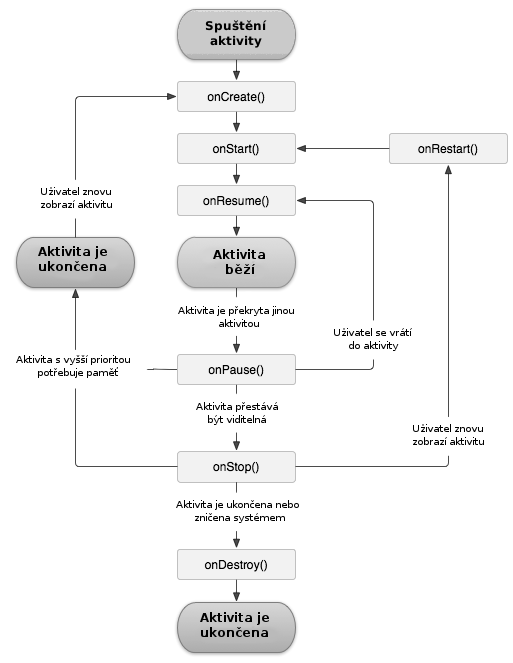
\includegraphics[scale=0.68]{images/lifecycleBW.png}}
\caption{Životní cyklus aktivit.} \label{lifecycle}
\end{figure}
\subsection{Intenty}
Intenty jsou základními komunikačními prvky mezi jednotlivými komponentami aplikace. Je to tedy objekt třídy Intent, který slouží pro spuštění aktivity nebo služby a dokáže přenášete jednoduchá data mezi těmito komponentami. Rozdělujeme je na explicitní a implicitní:
\newpage
\begin{itemize}
\item explicitní - Používají se ke spuštění jedné konkrétní aktivity. Systém přesně ví, jak reagovat.
\definecolor{lightGrey}{RGB}{250,250,250}

\begin{lstlisting}[language=Java,
title=Ukázka explicitního intentu.,
basicstyle=\ttfamily\small\color{black},
commentstyle=\itshape,
keywordstyle=\color{Blue},
showstringspaces=false,
frame=lines,
backgroundcolor=\color{lightGrey}
]
Intent i = new Intent(context, CameraActivity.class);
\end{lstlisting}
\item implicitní - Používají se v případě, kdy je jasné co má být provedeno, ale není definované jak danou činnost provést. To necháme na systému.
\begin{lstlisting}[language=Java,
title=Ukázka implicitního intentu.,
basicstyle=\ttfamily\small\color{black},
commentstyle=\itshape,
keywordstyle=\color{Blue},
showstringspaces=false,
frame=lines,
backgroundcolor=\color{lightGrey}
]
Uri uri = Uri.parse("http://www.spotting.com");
Intent i = new Intent(Intent.ACTION_VIEW, uri);
startActivity(i);
\end{lstlisting}
Na příkladu můžete vidět otevření webové stránky z aktivity pomocí nějakého internetového prohlížeče.
\end{itemize}
\subsection{Poskytovatelé obsahu}
Jak jsem zmiňoval výše, lze přes intenty posílat a přijímat menší množství dat, které se ale nehodí pro větší objemy dat. Z tohoto důvodu jsou v systému poskytovatelé obsahu, kteří jsou určení ke sdílení dat mezi jednotlivými aplikacemi v celém systému. Systém je dodáván s poskytovateli obsahu pro některé zakladní typy dat a řadu z nich najdeme v balíčku Android.provider. Jestliže chceme sdílet některá data, je to možné dvojím způsobem:
\begin{enumerate}
\item a to vytvořením vlastního poskytovatele obsahu za pomocí třídy contentProvider\footnote[8]{Komponenta spravující sdílená aplikační data.}.
\item nebo využitím stávajícího poskytovatele obsahu, kdy musí poskytovat stejný typ dat a také musíte mít povolený přístup pro zápis.
\end{enumerate}
\subsection{Služby}
Aktivity a poskytovatelé obsahu jsou entity s krátkou životností, které lze kdykoliv vypnout. Proto existují služby, které jsou navrženy tak, aby mohli provádět dlouhotrvající operace na pozadí. Služby neposkytují GUI a nejsou proto vázány na grafické rozhraní aplikace. Např. lze tedy přehrávat hudbu, i když aktivita, při které bylo spuštěno přehrávání, už byla ukončena.
\subsection{Přijímače}
Komponenta odvozená od třídy android.app.BroadcastReceiver slouží k naslouchání oznámení. Poté umožňuje reagovat aplikaci na nějakou událost, která nemusela vzniknout v rámci aplikace, ale mohla vzniknout systémem nebo jinou aplikací. Příkladem může být oznámení o příchodu sms zprávy.
\newpage
\section{Návrh aplikace}
%V této části se budu zabývat programátorskými aspekty práce. Zaměřuje se na architekturu aplikace, dále popisuje knihovny použité při tvorbě aplikace.
V této části se budu zabývat návrhem aplikace, která mi poskytne následné informace k samotné implementaci. Zaměřuji se na popis diagramu případu užití, návrhu architektury a popisu použitých knihoven.
\subsection{Diagram případů užití}
Diagram případu užití znázorněn na obr. \ref{diagram} popisuje funkční požadavky na
\begin{figure}[ht]
\centerline{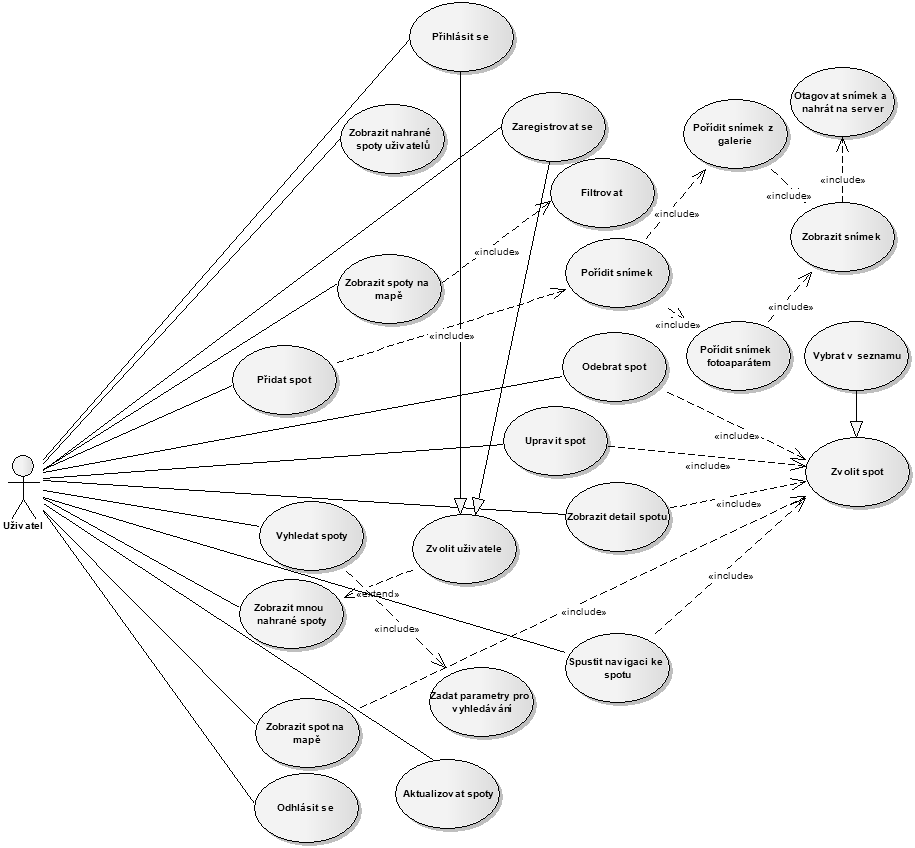
\includegraphics[scale=0.5]{images/spotting-diagramBW.png}}
\caption{Diagram případů užití aplikace.} \label{diagram}
\end{figure}
systém. Zobrazuje jednotlivé případy užití, které nám znázorňují interakce mezi uživatelem  aplikace a aplikací samotnou.
\begin{itemize}
\item Přihlásit se - funkce na přihlášení do sytému, která se spustí při prvním spuštění, pokud uživatel jíž není přihlášen.
\item Zaregistrovat se - funkce pro vytvoření účtu do systému.
\item Zobrazit nahrané spoty uživatelů - zobrazení nahraných spotů probíhá automaticky po zapnutí aplikace, jestliže se uživatel již někdy přihlásil do systému.
\item Aktualizovat spoty - po stisknutí aktualizovacího tlačítka se obnoví seznam nahraných spotů.
\item Zobrazit spot na mapě - vyvolá novou aktivitu pro zobrazení spotu na mapě, kdy se přímo přiblíží pohled na vybraný spot.
\item Zobrazit detail spotu - umožňuje zobrazit detailní popis po kliknutí na spot ze seznamu zobrazených.
\item Spustit navigaci ke spotu - spuštění této funkce se vyvolá pomocí implicitního intentu, který převezme některá z aplikací pro navigaci.
\item Zobrazit spoty na mapě - vyvolá novou aktivitu se zobrazenými skate spoty na mapě. Lze dále přepínat mezi spoty pro cyklisty a bruslaře.
\item Přidat spot - tato funkce vyvolá novou aktivitu, kdy se spustí fotoaparát. Zde lze pořídit snímek dvojím způsobom a to vyfotografováním, nebo výběrem z galerie. Po pořízení snímku ve čtvercovém formátu se spustí nová aktivita se zobrazeným snímkem. Jestliže se nám pořízený snímek nepovedl můžeme se vrátit zpět pro znovu vytvoření, nebo pokračovat a spustit novou aktivitu pro otagování a nahrání vytvořeného spotu na server.
\item Vyhledat spoty - tato funkce slouží pro vyhledávání, kdy zadáním určitých parametrů ji upřesníme např. zvolíme vzdálenost do 5km a zaškrtneme políčko skate, tím se nám vyvolá nová aktivita se seznamem skate spotů do dané vzdálenosti.
\item Zobrazit mnou nahrané spoty - zobrazím v seznamu všechny uživatelem nahrané spoty.
\item Odebrat spot - umožňuje po kliknutí na spot ze seznamu uživatelem nahraných jeho odstranění.
\item Upravit spot - umožňuje po kliknutí na spot ze seznamu uživatelem nahraných změnit některé údaje.
\item Odhlásit se - funkce na odhlášení ze systému.
\end{itemize}
\begin{figure}[ht]
\centerline{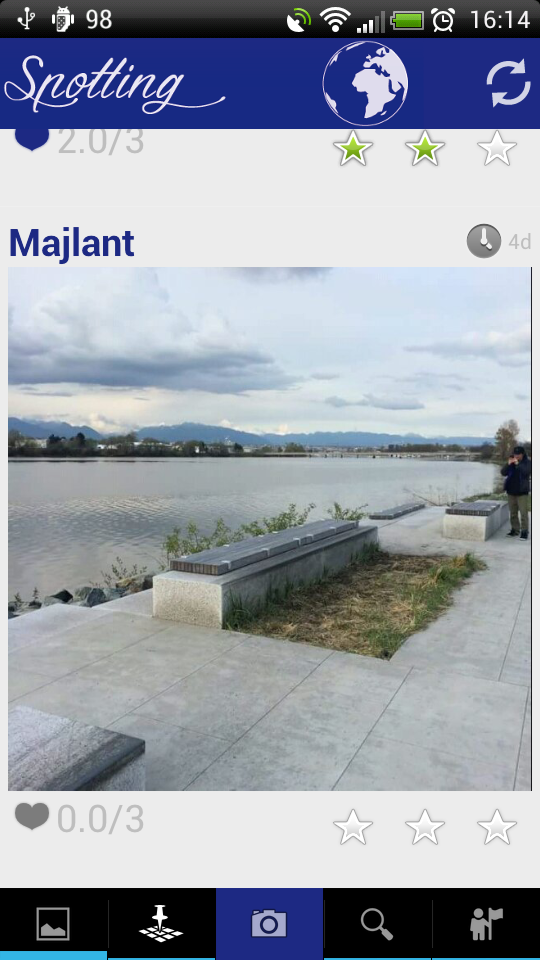
\includegraphics[scale=0.2]{images/spotting.png} 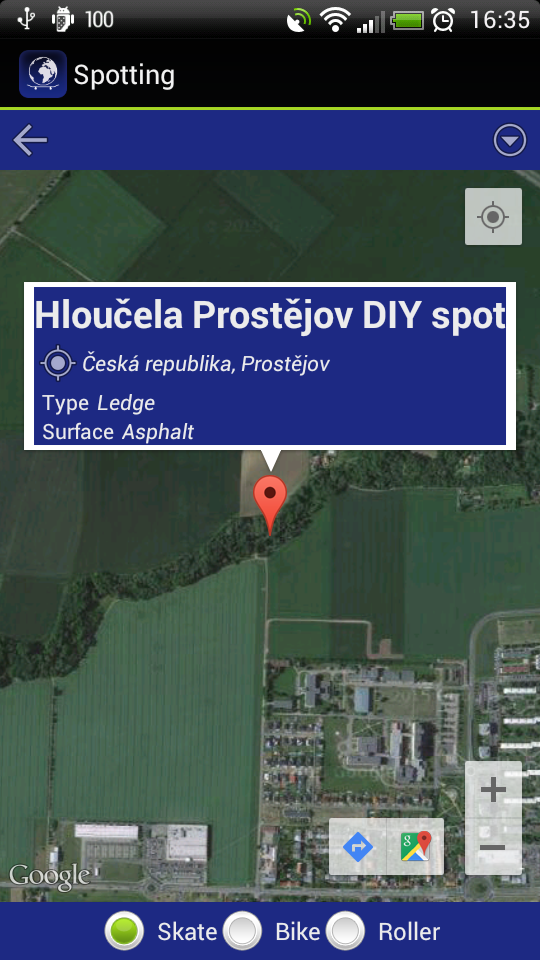
\includegraphics[scale=0.2]{images/spotting2.png} 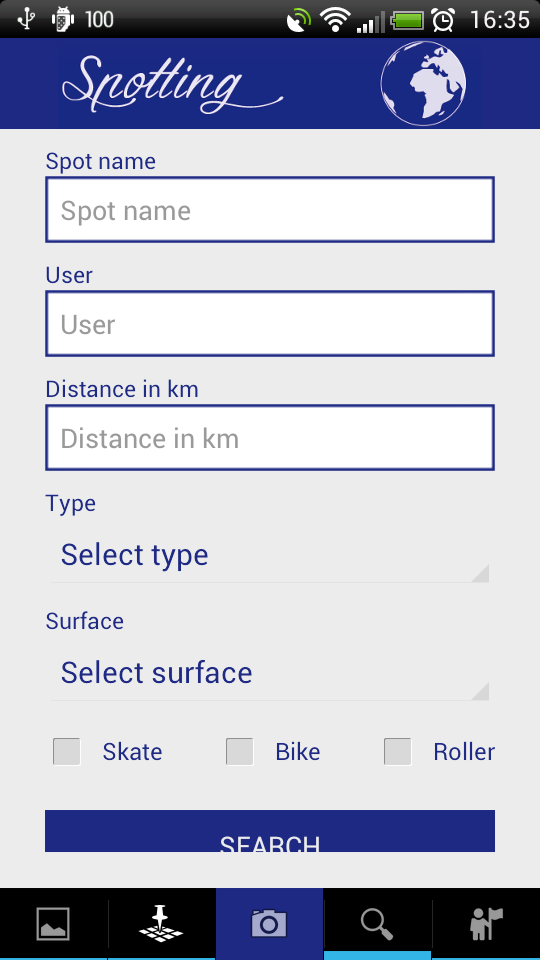
\includegraphics[scale=0.2]{images/spotting3.png}}
\caption{Obrazovka se seznamem spotů (vlevo), mapy se spoty (uprostřed) a pro vyhledávání (vpravo).} \label{screens}
\end{figure}
\subsection{Architektura aplikace}
Součástí systému je serverová část a klientská android aplikace komunikující s tímto serverem. Komunikace mezi android klientem a serverem je skrz REST\footnote[9]{Representational State Transfer - architektura webových aplikací, která nám umožňuje přistupovat k datům.} služby. Jako datové úložiště je zvoleno MySQL.

Využívám tedy třívrstvé architektury, kdy je aplikace rozdělena na to co uživatel vidí a na to, co se odehrává na pozadí na straně serveru.

Vrstvy architektury:
\begin{itemize}
\item Prezentační vrstva - Klientská mobilní aplikace pro platformu Android.
\item Aplikační vrstva - Prostředník mezi prezentační a datovou vrstvou. Je tvořena PHP skripty společně s SQL příkazy, které běží na webovém serveru. Zvolil jsem free hostingový server Endora.cz, který splňoval nejlépe mé požadavky např. bezplatnou registraci domény III. řádu, bezplatný hosting a podporu MySQL databází.
\item Datová vrstva - Její úlohou je ukládání dat do perzistentního uložiště. V mém systému, jak jsem již zmiňoval byla zvolena relační databáze MySQL.
\end{itemize}
Výhodou zvolené architektury je rozdělení výkonu mezi zařízení uživatele a serveru. Díky tomuto může aplikace běžet i v low-end zařízeních. Dále umožňuje nezávislé správy jednotlivých vrstev.
\subsection{Použité knihovny}
Při vývoji byla použita i řada externích knihoven, které si v této kapitole rozebereme.
\subsubsection{Volley}
\label{volley}
Je knihovna vyvíjená společností Google, která slouží pro snadnější a hlavně rychlejší používání síťových požadavků. Mezi její výhody patří automatické plánování síťových požadavků, umožnění více souběžných připojení k síti, poskytnutí paměťového cachování a také umožňuje zrušit pouze jednu nebo všechny žádosti.

Její nevýhodou je, že nedokáže stahovat větší soubory, z důvodu, že udržuje všechny odpovědi v paměti.\cite{volley}
\subsubsection{Google Play Services}
Google Play Services je soubor služeb, jejichž hlavním účelem je ulehčení práce vývojářům. V této aplikaci využívám služby pro získání polohy od nejlepšího poskytovatele a přístup k Google Maps.

Jestliže knihovna Google Play Services není nainstalována na zařízení, tak služby na daném zařízení nebudou fungovat.\cite{services}


Další použité knihovny (httpclient-4.3.6, httpcore-4.3.3, httpmime-4.3.6) využívané při odesílání dat s ukazatelem průběhu na server viz. kapitola \ref{knihovny}.
\newpage
\section{Implementace}
V této části se budu zabývat programátorskými aspekty práce. Je zde popsána většina vytvořených tříd. Dále budu dělit třídy podle jejich typu.
\subsection{Activity}
O aktivitách jsem se již bavil v kapitole \ref{aktivity}, nyní si popíšeme jednotlivé aktivity použité v aplikaci.
\subsubsection{Login}
Přihlašovací obrazovka, pomocí které se lze přihlásit do systému. Aktivita \verb+Login+ obsahuje dvě tlačítka (pro přihlášení a pro přepnutí do aktivity \verb+Registration+ pro založení účtu) a formulář (pro vyplnění údajů uživatele). K přihlášení je potřeba internetového připojení, z důvodu uložení dat o uživateli v MySQL databázi na straně serveru. O výměnu dat mezi klientskou aplikací a databází se stará PHP skript \verb+logAndReg.php+. Jejím úkolem je dostat požadavek od klienta, provést dotazy na databázi a odeslat odpověď zpět klientovi.

K síťovým požadavkům využívám knihovnu volley viz. \ref{volley}, která mi stahování dat ze serveru velice usnadňuje. Jinak bych musel např. stahovat data ve vlastním vlákně přes \verb+AsyncTask+. Po přijetí požadavku se vytvořené API připojí na databázi přes \verb+newConnection.php+ skript a zkontroluje, zda se předané údaje shodují s uživatelem v databázi a odešle za pomocí funkce \verb+json_encode+ klientovi odpověď zpět ve formátu JSON.
\begin{lstlisting}[title=Ukázka odpovědi s chybovou zprávou]
{
   "error":true,
   "error_msg":"Incorrect nick or password!"
}
\end{lstlisting}
\begin{lstlisting}[title=Ukázka odpovědi s úspěšným přihlášením]
{
   "error":false,
   "users_id":"157",
   "user":{
      "nick":"Majlant",
      "email":"jir.mil@centrum.cz"
   }
}
\end{lstlisting}

Po úspěšném přihlášení se nastaví za pomocí \verb+Shared preferences+\footnote[10]{Uložiště, kam lze ukládat nějaká data.}, že je uživatel již přihlášen.  Práci s ní má na starosti třída \verb+SPManager+. Dále se uloží data o uživateli do lokální databáze SQLite a spustí se aktivita \verb+Spotting+. 

Po znovu spuštění aplikace se již nemusíme přihlašovat. Funkce \verb+checkLogged+ provede kontrolu stavu přihlášení i v tzv. offline režimu.
\subsubsection{Registration}
Registrační obrazovka, pomocí které lze založit účet do systému. Obsahuje dvě tlačítka (pro zaregistrování a přepnutí do aktivity \verb+Login+) a formulář (pro vyplnění údajů uživatele) skládající se ze čtyř \verb+EditTextů+.

Registrace probíhá obdobně jako již bylo zmíněno u aktivity \verb+Login+. Před odesláním požadavku na server, se ale provede na straně klienta základní validace formuláře. Provede se kontrola vyplnění všech polí ve formuláři, validace e-mailu, kterou provádí funkce \verb+isValidEmail+, shody zadaných hesel a minimální délky hesla, která musí přesahovat délku pěti znaků.
\subsubsection{Spotting}
\verb+Spotting+ je hlavní aktivita obsahující pět záložek. Je to takový rozcestník funkcí aplikace.

Po prvním spuštění je volána metoda \verb+getSpots+, která požádá server o šest posledně nahraných spotů uživatelů. Odpověď je opět ve formátu JSON viz. ukázka na konci kapitoli \ref{lst:json}. Tu má na starosti \verb+fileDownload.php+ skript. Metoda \verb+doResponseSpots+ zpracuje odpověď, vytvoří instanci třídy \verb+SpotLoadAdapter+ viz. třída \ref{SpotLoadAdapter} a ta se nastaví jako adaptér pro ListView\footnote[11]{Rozložení zobrazující rolující seznam položek.} \verb+spotsInListView+. Poté je zobrazen seznam spotů, které můžeme procházet rolováním.

Další funkcí implementovanou v této třídě je vyhledávání. Komunikace se serverem je prováděna v metodě \verb+searchSpots+. Ta probíhá obdobně jako v předchozím odstavci. Jen se provádí se \verb+searchSpots.php+ skriptem. Pro prohledávání textů v MySQL databázi využívám jednoduchého operátoru LIKE. Umožňuje vyhledávat řetězce jen dle části textu. Lze i vyhledávat do určité vzdálenosti. K tomu využívám Haversinův vzorec. Ten dokáže mezi dvěma body na zeměkouli dané zeměpisnou délkou a šířkou vypočítat jejich vzdálenost.\cite{haversine} Výše popsaná problematika je implementovaná ve funkci \verb+getSpotsByUser+. Ta najde záznamy v tabulce podle vytvořeného dotazu a údajů uživatele.
\newpage
\begin{lstlisting}[title=Ukázka odpovědi PHP skriptu fileDownload.php,
label={lst:json}]
[
   {
      "tag":"download",
      "error":false,
      "spot":{
         "like":"false",
         "my_rate":-1,
         "img_name":"IMG_20150716_073244.jpg",
         "user_name":"Jirka",
         "spot_name":"test",
         "type":"Park",
         "surface":"Asphalt",
         "bike":"true",
         "roller":"false",
         "skate":"false",
         "description":"",
         "latitude":"49.5902812",
         "longitude":"17.2494468",
         "number_rate":"0",
         "date":"2015-07-16 07:33:20",
         "rate":"0"
      },
      "spot_id":"241"
   }
]
\end{lstlisting}
\subsubsection{Map}
\label{map}
Aktivita \verb+Map+ znázorňující obrazovku s mapou. Pro přidání map do aplikace jsem využil \verb+Google Maps Android API+. Toto API automaticky obsluhuje přístup ke Google Maps serverům, stahování dat, rekce na gesta uživatele a zobrazení samotné mapy.\cite{maps}

Mapa je zobrazena ve fragmentu třídy \verb+com.google.android.gms.maps.MapFragment+. Další funkcí mimo prosté zobrazení je možnost změny typu mapy na satelitní, normální či s terénem, kterou provádí metoda \verb+myClickHandler+. Dalším stěžejním bodem bylo přidání bodů (spotů) tzv. \verb+markery+ do mapy na zvolených místech a vytvoření informačního okna, které se zobrazí po kliknutí na kterýkoli z nich.
Přidání se implementovalo jednoduchým voláním \verb+GooleMap.addMarker+. Pro vlastní informační okno byla potřeba vytvořit \verb+InfoWindowAdapter+ třídu, přepsat \verb+getInfoContents+, který poskytuje vlastní obsah a zavolat \verb+GooleMap.setInfoWindowAdapter+ pro nastavení vlastního \verb+InfoWindowAdapter+.

Zobrazené spoty lze i filtrovat dle druhu sportu. Ke stahování informací o spotech je opět využita knihovna volley komunikující s \verb+downloadAllSpots.php+ skriptem.
\subsubsection{MapSpot}
Aktivita \verb+MapSpot+ znázorňující obrazovku s mapou a vyznačeným spotem na ní. Dále se s ní nebudu zabývat. Informace o ní jsou velice obdobné jako v kapitole \ref{map}.
\subsubsection{CameraActivity}
Aktivita \verb+CameraActivity+ znázorňující obrazovku vlastního fotoaparátu. Aktivita slouží k získání obrázku (spotu). K tomu slouží dva způsoby:
\begin{itemize}
\item Z galerie - Po vyběru této možnosti se uživatelovi naskytne možnost vybrat si obrázek již uložený v jeho zařízení. Při implementaci využívám implicitního \verb+Intentu+ viz. následující ukázka.
\definecolor{lightGrey}{RGB}{250,250,250}

\begin{lstlisting}[language=Java,
title=Následujícím kódem použitý v aplikaci se vyvolá nabídka pro výběr snímku z galerie.,
basicstyle=\ttfamily\small\color{black},
commentstyle=\itshape,
keywordstyle=\color{Blue},
showstringspaces=false,
frame=lines,
backgroundcolor=\color{lightGrey}
]
Intent picPathIntent = new Intent(Intent.ACTION_PICK);
picPathIntent.setType(getDataImageType());
startActivityForResult(picPathIntent, SELECT_PHOTO);
\end{lstlisting}
Konstanta \verb+Intent.ACTION_PICK+ říká, že se jedná o požadavek pro získání adresy dat. Ty jsou reprezentované pomocí \verb+Uri+ třídy \verb+android.net.Uri+. Dále za pomocí \verb+setType+ bylo specifikováno, o jaký typ dat se jedná. Ke spuštění byla použita metoda \verb+startActivityForResult+ a je tedy zřejmé, že poté co nově spuštěná aktivita dokončí zadaný úkol, musí předat výsledek zpět (\verb+Uri+) rodičovské aktivitě. K tomu bylo ještě zapotřebí doimplementovat metodu \verb+onActivityResult+, pro zpracování výsledku. Z důvodu, že v aplikaci jsou využívány obrázky ve čtvercovém formátu, je po získání výsledku volána metoda \verb+performCrop+. V ní se nastaví parametr akce s názvem \verb+"com.android.camera.action.CROP"+ a další požadované parametry. Opět v metodě \verb+onActivityResult+ se získá výsledek, nyní akcí pro ořezání obrázku.
\item Z kamery - Tato možnost umožní vyfotografování obrázku. Pro vytvoření vlastního fotoaparátu používám balíček \verb+android.hardware.Camera+, který obsahuje rozhraní pro jednotlivé kamery zažízení se systémem Android. Nyný již lze využívat novější \verb+android.hardware.camera2+ API, ale pouze pro úroveň API 21 a výše. Následně popíši některé základní kroky, které byly použity k vytvoření vlastního fotoaparátu. Nejdříve je získána instance objektu \verb+Camera+ metodou \verb+getCameraInstance()+. Poté byla vytvořena instance vlastní třídy \verb+CameraPreview+, která rozšiřuje \verb+SurfaceView+ a implemnetuje \verb+SurfaceHolder.Callback+ rozhraní. Tato třída umožňuje zobrazit náhled obrazu z fotoaparátu a za pomocí zpětných volání zachytit vytvoření a zrušení \verb+View+. Nyní připojíme oblast pro vykreslování k fotoaparátu metodou \verb+Camera.setPreviewDisplay()+ s parametrem instance třídy \verb+SurfaceHolder+. Nakonec byla potřeba zahájit zobrazování snímků z fotoaparátu metodou \verb+Camera.startPreview()+. Před pořízování snímků, bylo nutností nastavení jejich kvality. To se provádí přes objekt \verb+Camera+ v metodě \verb+setBestQualityCamera()+. Teď nám již nic nebrání v jejich pořízení. Načtení obrázků provádím pomocí metody \verb+Camera.takePicture()+. V aplikaci využívám snímky ve formátu JPEG, z toho důvodu implmentuji rozhraní \verb+Camera.PictureCallback+ pro příjem obrazových dat. Posledním stežejním je ořezání obrázku do čtvercového formátu a uvolnění kamery. Při vývoji první problematiky jsem se potýkal s problémem, kdy byla vyvolávána vyjímka \verb+java.lang.OutOfMemoryError+. Důvodem bylo, že zařízení se systémem Android mají omezené množství paměti pro každou aplikaci. Řešením problému bylo přidat do souboru manifest \verb+android:largeHeap="true"+ a tím byla navýšena přidělená paměť aplikace, která je pro práci s obrázkami téměř nutností. Nesmíme opomenout na uvolnění kamery, z důvodu, že je to zdroj, který je sdílený mezi aplikacemi. Uvolnění provádím metodou \verb+stopPreviewAndFreeCamera()+ implementovanou v třídě \verb+CameraPreview+.\cite{camera}
\end{itemize}
\subsubsection{ShowPhoto}
\verb+ShowPhoto+ je aktivita znázorňující obrazovku s obrázkem pořízený v \verb+CameraActivity+. Je to takový prostředník mezi dvěmi aktivitami. Samotný obrázek je uložen na zařízení v externí paměti. Pro jeho získání je mezi aktivitami předávána cesta k souboru, která je specifikována absolutní cestou.
\subsubsection{AddSpot}
\label{knihovny}
\verb+AddSpot+ slouží pro otagování a odesílání spotů na server. V této sekci se zabývám implementací získání geografických souřadnic (zeměpisná šířka/zeměpisná délka) a odesílání dat na server.
\begin{itemize}
\item Určení polohy - pro určení polohy lze využít dvě funkce, kdy souřadnice získáme pomocí:
\begin{itemize}
\item Zadáním adresy: pro získání zeměpisné šířky a délky z adresy využívám třídu \verb+Geocoder+ implementovanou v třídě \verb+LocationFromAddressDialog+ rozšiřující \verb+AlertDialog.Builder+. Tento proces je nazýván geokodování.\cite{geocoder}
\item Poskytovatele polohy GPS a siťového poskytovatele: Android doporučuje využívat jejich nejnovější API zvané \verb+Google Play services location API+, které jsem se rozhodl i využívat. To nabízí snadnější a přesnější určování polohy. Říkají, že by měla být i snížená spotřeba baterie. Tyto služby jsou poskytované prostřednictvím Google Play sloužeb. API vyžaduje nejříve integrovat Google Play služby pomocí \verb+GoogleApiClient+. To provádím metodou \verb+buildGoogleApiClient()+ volanou v \verb+onCreate()+. Poté je připojena metodou \verb+connect()+ v \verb+onStart()+. Jenž je \verb+GoogleApiClient+ úspěšně připojen, tak v \verb+onConnected+ zaregistrujeme \verb+LocationListener+ pro aktualizaci polohy metodou \verb+startLocationUpdates()+. Odpojení je provedeno metodou \verb+disconnect()+ v \verb+onStop()+.\cite{location}
\end{itemize}
\item Odesílání dat na server - V této části se zabývám odesíláním binárních dat s ukazatelem průběhu na server. Ke komunikaci se server nevyužívám knihovnu volley jako doposud. Nehodí se pro odesílání větších souborů a nepodporuje ani ukazatel průběhu (progress bar). Pro odesílání využívám metody POST protokolu HTTP\footnote[12]{Protokol určený pro přenos HTML dokumentů mezi klientem a serverem.} z balíčku \verb+org.apache.http+. HTTP komunikace nelze provádět v UI vlákně aplikace. Pro tyto účely jsem rozšířil třídu \verb+Upload+, ve které je implementována veškerá logika komunikace o třídu \verb+AsyncTask+. Nyní již je veškerá komunikace prováděna na pozadí a nezasahuje do běhu UI vlákna. Samotná třída \verb+AsyncTask+ implementuje několik metod \verb+onPreExecute+, \verb+doInBackground+, \verb+onPostExecute+ a \verb+onProgressUpdate+. Odesílání se spustí v hlavním vlákně pomocí metody \verb+execute+ a zavolá se metoda \verb+onPreExecute+, v které se zobrazí ukazatel průběhu. Po zobrazení ukazatele průběhu se vykoná komunikace se serverem implementována v metodě \verb+uploadFile+, která je spustěná v \verb+doInBackground+. Po dokončení této metody se zavolá \verb+onPostExecute+. V ní se zruší ukazatel a spustí se aktivita se seznamem spotů. %Ještě se podrobněji podíváme, jak probíhala komunikace v \verb+doInBackground+. Nejdříve jsem si vytvořil instanci třídy \verb+DefaultHttpClient+. Vytvořil jsme nového klienta. Dále jsem vytvořil instanci třídy \verb+HttpPost+
\end{itemize}
\subsubsection{Search}
Aktivita \verb+Search+ znázorňující obrazovku se seznamem spotů (\verb+ListView+) s nastaveným adaptérem \verb+SpotLoadAdapter+ viz. kapitola \ref{SpotLoadAdapter}. 
\subsection{Adaptéry}
Třída adaptér se využívá jako most mezi \verb+AdapterView+ (v této práci využívám \verb+ListView+) a daty, která dané \verb+View+ zobrazují. Stará se o vytváření jednotlivých položek \verb+View+ v seznamu, dle vlastního rozložení prvků. \cite{adapter}
\subsubsection{SpotLoadAdapter}
\label{SpotLoadAdapter}
Pro vytvoření \verb+ListView+ se seznamem spotů, je vždy potřeba vytvořit instanci třídy \verb+SpotLoadAdapter+ s parametry \verb+Activity+ a seznamem spotů (\verb+List<SpotModel>+). Ta se stará o předání dat a jejich zobrazení v \verb+ListView+. Jedna položka v seznamu se skládá ze tří \verb+TextView+ a jednoho \verb+ImageView+, \verb+ImageButtonu+ a \verb+RatingBaru+. Fotky zobrazované v \verb+ImageView+ se stahují ze serveru. Po jejich přidání výkon prohlížení výrazně poklesl, aplikace byla téměř nepoužitelná. Řešení jsem našel v tomto tutoriálu \cite{cache}. Problém byl v tom, že se v paměti udržoval pouze zobrazovaný a při srolování na jiný se musel nejdříve stáhnout. To je velice neefektivní a proto byla vytvořena vyrovnávací paměť\footnote[13]{Pamět sloužící k dočasnému uschování dat.} na SD kartě v adresáři \verb+/mnt/sdcard/spottingCache+. Vše je implementované v následujících třídách:
\begin{itemize}
\item \verb+SpotImageLoader+ - Slouží pro stahování obrázků ve vlastním vlákně z URL\footnote[14]{Adresa určující umístění dokumentu na internetu.} adresy, nebo mohou být načteny z vyrovnávací paměti, pokud již byly staženy dříve.
\item \verb+FileCache+ - Slouží k vytvoření adresáře na SD kartě, získání souboru z adresáře pomocí URL obrázku a také můžeme použít metodu \verb+clear+ pro odstranění všech souborů z adresáře.
\item \verb+MemoryCache+ - Slouží k nastavení limitu velikosti složky vyrovnávací paměti a také k jejímu vymazání.
\item \verb+Utils+ - Slouži k překopírování staženého obrázku do paměti metodou \verb+copyStream+.
\end{itemize}
\subsubsection{DetailsListViewAdapter}
Jednoduchý adaptér, které slouží k vytvoření a nastavení dvou \verb+TextView+. Adaptér se nastavuje pro \verb+ListView+ implementovaný v třídě \verb+SpotDetailsDialog+ viz. kapitola \ref{details}.
\subsection{Dialogy}
Dialog je malé vyskakovací okno, které se nejčastěji využívá ke sdělení nějaké informace uživateli, k nějakému rozhodnutí (souhlas/odmítnutí) či, aby vyčkal na dokončení prováděné úlohy. Android nabízí celou řadu předdefinovaných jednoduchých dialogů. V aplikaci využívám např.
\begin{itemize}
\item \verb+ProgressDialog+, který dává uživateli najevo, že aplikace pracuje.
\item \verb+AlertDialog+, který je jeden z nejpoužívanějších dialogů. Umožňuje zobrazit titulek, až tři tlačítka a nějaký obsah, který může mít vlastní rozvržení.
\item a další.
\end{itemize}
V aplikaci byly potřeba i složitější dialogy. K tomu jsem si vytvořil vlastní dialogy rozšiřující třídu \verb+Dialog+ s definováním vlastního rozvržení. Jedná se o dialog pro změnu hesla, úpravu údajů o spotu, zobrazení informací a další. Následuje popis některých dialogů.
\subsubsection{ChangePassDialog}
\verb+ChangePassDialog+ je vlastní dialog využívající se ke změně přihlášeného uživatele do aplikace. Zobrazuje tři \verb+EditTexty+ (pro zadání starého a nového hesla) a dvě tlačítka (pro potvrzení požadavku nebo zavření dialogu). V samotné třídě je implementována komunikace se serverem knihovnou volley v metodě \verb+uploadChangePass+.
\subsubsection{SpotDetailsDialog}
\label{details}
\verb+SpotDetailsDialog+ je dialog zobrazující seznam (\verb+ListView+) nastavený na instanci \verb+DetailsListViewAdapter+ adaptéru. Ten je vytvořen s parametry \verb+Context+ a seznamem \verb+ArrayList+, ve kterém jsou obsažené data pro vypsání. Ty jsou vytvářeny v metodě \verb+createModels+. Samotný dialog tedy zobrazuje veškeré informace o spotu.
\subsubsection{DialogSpot}
\verb+DialogSpot+ se zobrazí po kliknutí na kterýkoli nahraný spot ze seznamu spotů uživatelů. Obsahuje čtyři tlačítka:
\begin{itemize}
\item pro zobrazení spotu na mapě - tato funkce je implementována v metodě \verb+setMapEvent+.
\item pro zobrazení informací o spotu - tato funkce je implementována v metodě \verb+setDetailsEvent+.
\item pro spuštění navigace od uživatelové polohy ke spotu - tato funkce je implementována v metodě \verb+setNavigationEvent+.
\item pro zavření dialogu - tato funkce je implementována v metodě \verb+setCancelEvent+.
\end{itemize}
\subsubsection{DialogEdit}
\verb+DialogEdit+ se zobrazí po kliknutí na některý spot ze seznamu uživatele nahraných. Slouží k úpravě či změně údajů k danému spotu. Všechna políčka pro úpravu jsou nastavená dle předchozího zadání údajů v konstruktoru voláním metod, jako jsou např. \verb+setNickView+ pro jméno, \verb+setTypeView+ pro typ, \verb+setSurfaceView()+ pro povrch a další. Komunikaci se serverem zprostředkovávaná přes \verb+editSpot.php+ skript je implementovaná v metodě \verb+editUserSpot+ knihovnou volley.
\subsection{Ostatní třídy}
V této kapitole se budu zabývat třídami, které nelze dělit dle typu.
\subsubsection{SpotModel}
\verb+SpotModel+ je třída implementující rozhraní \verb+Parcelable+. Byla vytvořena jako dotavý nosič. Obsahuje proměnné pro uchování informací o spotu. Využívá se tedy pro sdílení dat mezi aktivitami, kdy nám nestačí primitivní datové typy. Data je možné poslat spouštěnné aktivitě pomocí záměru.
\begin{lstlisting}[language=Java,
title=Následujícím kódem použitý v aplikaci se spustí aktivita \lstinline!Search! se seznamem objektů \lstinline!SpotModel!.,
basicstyle=\ttfamily\small\color{black},
commentstyle=\itshape,
keywordstyle=\color{Blue},
showstringspaces=false,
frame=lines,
backgroundcolor=\color{lightGrey}
]
Intent i = new Intent(context, Search.class);
i.putParcelableArrayListExtra(Search.SPOTS_LIST, searchSpots);
startActivity(i);
\end{lstlisting}

\begin{lstlisting}[language=Java,
title=Tímto kódem naopak předaný seznam získáme zpět.,
basicstyle=\ttfamily\small\color{black},
commentstyle=\itshape,
keywordstyle=\color{Blue},
showstringspaces=false,
frame=lines,
backgroundcolor=\color{lightGrey}
]
Intent i = this.getIntent();
spots = i.getParcelableArrayListExtra(SPOTS_LIST);
\end{lstlisting}
\subsubsection{Config}
Třída obsahující řetězcové konstanty URL adres.
\subsubsection{DetailsModel}
Třída, která byla vytvořena pro zapouzdření proměnných a metod do jednoho objektu.
\subsubsection{AppController}
\verb+AppController+ rozšiřující třídu \verb+Application+. Je to třída, která potřebuje udržet globální stav. Využívá se při práci s knihovnou volley, kdy udržuje základní objekty a frontu požadavků. 
\cite{volley-singleton}
\newpage
\section{Závěr}
Cílem práce bylo vytvořit aplikaci pro mobilní platformu Android, která umožní uživatelům vyhledání míst pro skateboardery, bikery a bruslaře a následné zveřejnění pomocí služby Google Play.

Jelikož s programováním pro tuto platformu jsem neměl žádné zkušenosti, tak to bylo pro mě velikým přínosem. Za hlavní přínos při tvorbě této práce pokládám nastudování a vyzkoušení nových technologií. Vyzkoušel jsem si některé nástroje z balíčku SDK, seznámil jsem se s vývojem Android aplikací, z jakých sestávají komponent či jejich životního cyklu. V neposlední řadě práci s některými poskytovanými funkcemi jako je např. Google Maps Android API pro práci s mapami, Google Play services location API pro určení polohy a další.

Mezi další náměty pro možné vylepšení aplikace je využití Facebook SDK. To umožní snadnější přihlášení do aplikace přes uživatelův Facebook účet a využití funkce sdílení na sociální síť Facebook. Dále by bylo vhodné obohatit aplikaci o možnost okomentování spotů, přidání dalších prvků pro umožnění snadnějšího vyhledávání na základě pozdějších požadavků uživatelů.
\newpage
\begin{thebibliography}{1} %při použití psát \cite{vobecky} apod
\bibitem{historie} Google Buys Android for Its Mobile Arsenal. In: \emph{Businessweek - Business News, Stock market \& Financial Advice} [online]. 16. 8. 2005 [cit. 2. 4. 2015]. Dostupné
z: \url{http://www.bloomberg.com/bw/stories/2005-08-16/google-buys-android-for-its-mobile-arsenal}
\bibitem{architektura} Android (operating system). In: \emph{Wikipedia, the free encyclopedia} [online]. 29. 6. 2012 [cit. 2. 4. 2015]. Dostupné z: \url{http://en.wikipedia.org/wiki/File:Android-System-Architecture.svg}

\bibitem{volba} Google Inc. Android Platform Version. In: \emph{Android Developers}
[Online]. 2. 3. 2015 [Citace: 3. 4. 2015]. Dostupné z: \url{http://developer.android.com/about/dashboards/index.html#Platform}

\bibitem{studio} Google Inc. Android Studio In: \emph{Android Developers}
[Online]. 2015 [Citace: 13. 5. 2015]. Dostupné z: \url{http://developer.android.com/tools/studio/index.html}

\bibitem{eclipse} Google Inc. Eclipse with ADT In: \emph{Android Developers}
[Online]. 2015 [Citace: 13. 5. 2015]. Dostupné z: \url{http://developer.android.com/tools/help/adt.html}

\bibitem{slozeni} GRANT Allen \emph{Android 4}
	Brno: Computer Press, 2013.
		[Citace: 13. 5. 2015]

\bibitem{volley} Google Inc. Volley library In: \emph{Android Developers}
[Online]. 2015 [Citace: 14. 7. 2015]. Dostupné z:
\url{https://developer.android.com/training/volley/index.html}

\bibitem{services} Google Inc. Google Play Services In: \emph{Android Developers}
[Online]. 2015 [Citace: 14. 7. 2015]. Dostupné z:
\url{https://developers.google.com/android/guides/overview#the_google_play_services_client_library}

\bibitem{adapter} Google Inc. Adapter In: \emph{Android Developers}
[Online]. 2015 [Citace: 17. 5. 2015]. Dostupné z: \url{http://developer.android.com/reference/android/widget/Adapter.html}

\bibitem{maps} Google Inc. Google Maps Android API v2 In: \emph{Android Developers}
[Online]. 14. 7. 2015 [Citace: 19. 7. 2015]. Dostupné z: \url{https://developers.google.com/maps/documentation/android/intro}

\bibitem{camera} Google Inc. Camera In: \emph{Android Developers}
[Online]. 2015 [Citace: 20. 7. 2015]. Dostupné z: \url{http://developer.android.com/guide/topics/media/camera.html#considerations}

\bibitem{geocoder} Google Inc. Geocoder In: \emph{Android Developers}
[Online]. 17. 7. 2015 [Citace: 21. 7. 2015]. Dostupné z: \url{http://developer.android.com/reference/android/location/Geocoder.html}

\bibitem{location} Google Inc. Google Play services location API In: \emph{Android Developers}
[Online]. 2015 [Citace: 21. 7. 2015]. Dostupné z: \url{http://developer.android.com/training/location/index.html}

\bibitem{cache} Cache In: \emph{ANDROIDHIVE}
[Online]. 10. 7. 2012 [Citace: 23. 7. 2015]. Dostupné z: \url{http://www.androidhive.info/2012/07/android-loading-image-from-url-http/}

\bibitem{volley-singleton} Google Inc. Volley-Singleton In: \emph{Android Developers}
[Online]. 2015 [Citace: 24. 7. 2015]. Dostupné z:
\url{https://developer.android.com/intl/zh-cn/training/volley/requestqueue.html#singleton}

\bibitem{haversine} Haversine formula In: \emph{Wikipedia}
[Online]. 1. 7. 2015 [Citace: 24. 7. 2015]. Dostupné z:
\url{https://en.wikipedia.org/wiki/Haversine_formula}

\end{thebibliography}
\end{document}